% 2005 年全国卷Ⅰ理科第 18 题：直角梯形底面的四棱锥
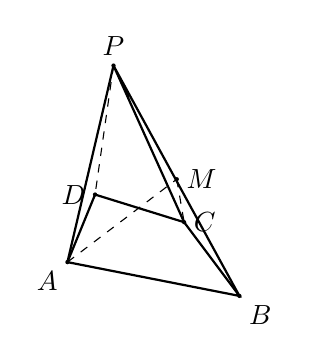
\begin{tikzpicture}[>=stealth,scale=0.78]
  \coordinate (A) at (0,0); \coordinate (B) at (2.8,-0.55);
  \coordinate (C) at (1.9,0.65); \coordinate (D) at (0.45,1.1);
  \coordinate (P) at (0.75,3.2); \coordinate (M) at (1.78,1.35);
  \draw[thick] (A)--(B)--(C)--(D)--cycle;
  \draw[thick] (P)--(A) (P)--(B) (P)--(C);
  \draw[dashed] (P)--(D) (A)--(M) (M)--(C);
  \fill (P) circle (1pt) node[above] {$P$};
  \fill (A) circle (1pt) node[below left] {$A$};
  \fill (B) circle (1pt) node[below right] {$B$};
  \fill (C) circle (1pt) node[right] {$C$};
  \fill (D) circle (1pt) node[left] {$D$};
  \fill (M) circle (1pt) node[right] {$M$};
\end{tikzpicture}
